\documentclass[tikz,border=15pt]{standalone}
\usepackage{amsmath,amssymb}
\usetikzlibrary{arrows.meta}

\begin{document}
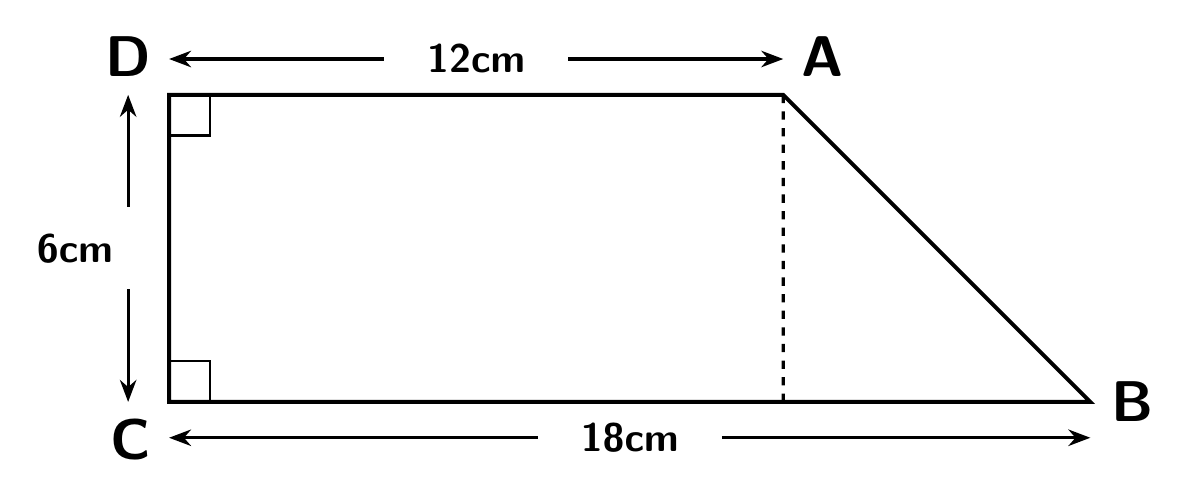
\begin{tikzpicture}[>=Stealth, scale=0.65]
    % Trapezium coordinates: C(0,0), B(18,0), A(12,6), D(0,6)
    \coordinate (C) at (0, 0);
    \coordinate (B) at (18, 0);
    \coordinate (A) at (12, 6);
    \coordinate (D) at (0, 6);
    
    % Draw boundary
    \draw[line width=1.4pt] (C) -- (B) -- (A) -- (D) -- cycle;
    
    % Dashed vertical altitude from A to base
    \draw[line width=1.2pt, dashed] (A) -- (12, 0);
    
    % Right angle symbols at D and C
    \draw[line width=1.0pt] (0, 5.2) -- (0.8, 5.2) -- (0.8, 6);
    \draw[line width=1.0pt] (0, 0.8) -- (0.8, 0.8) -- (0.8, 0);
    
    % Vertex labels in bold sans-serif
    \node[above left=3pt, font=\huge\sffamily\bfseries] at (D) {D};
    \node[above right=3pt, font=\huge\sffamily\bfseries] at (A) {A};
    \node[below left=3pt, font=\huge\sffamily\bfseries] at (C) {C};
    \node[right=4pt, font=\huge\sffamily\bfseries] at (B) {B};
    
    % Dimension callout for DA = 12cm (above)
    \draw[line width=1.1pt, <-] (0, 6.7) -- (4.2, 6.7);
    \draw[line width=1.1pt, ->] (7.8, 6.7) -- (12, 6.7);
    \node[font=\Large\sffamily\bfseries] at (6, 6.7) {12cm};
    
    % Dimension callout for CB = 18cm (below)
    \draw[line width=1.1pt, <-] (0, -0.7) -- (7.2, -0.7);
    \draw[line width=1.1pt, ->] (10.8, -0.7) -- (18, -0.7);
    \node[font=\Large\sffamily\bfseries] at (9, -0.7) {18cm};
    
    % Dimension callout for DC = 6cm (left)
    \draw[line width=1.1pt, <-] (-0.8, 6) -- (-0.8, 3.8);
    \draw[line width=1.1pt, ->] (-0.8, 2.2) -- (-0.8, 0);
    \node[left=2pt, font=\Large\sffamily\bfseries] at (-0.8, 3) {6cm};
    
\end{tikzpicture}
\end{document}
